\documentclass{article}
\usepackage{graphicx}
\usepackage{subcaption}  % For subfigures

\begin{document}

\title{Convolution of Step and Delta Functions with Various Kernels}
\author{Ankit}
\date{\today}
\maketitle

\section{Introduction}
This document presents the results of convolutions of step and delta functions with different kernels, including causal, symmetric, and shifted kernels. The convolution of these functions provides insights into how signals interact with different types of filters.

\section{Convolution Results}

\subsection{Step Function Convolution}
The following plots show the convolution of the step function $u(t)$ with different kernels.

\begin{figure}[h!]
    \centering
    \begin{subfigure}{0.45\textwidth}
        \centering
        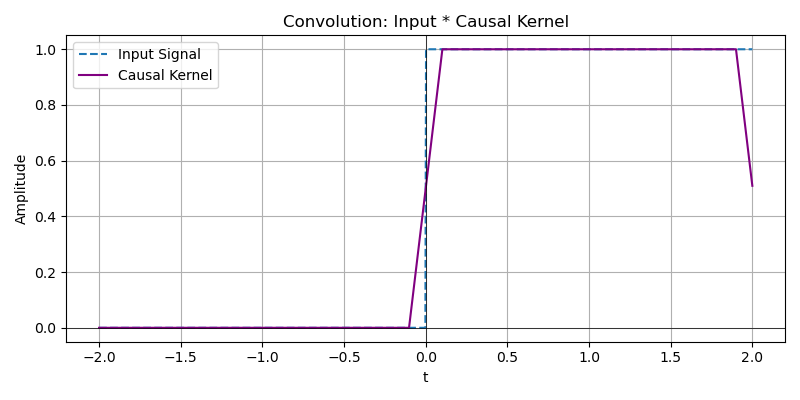
\includegraphics[width=\textwidth]{figs/1.png}
        \caption{Convolution with Causal Kernel}
    \end{subfigure}
    \hfill
    \begin{subfigure}{0.45\textwidth}
        \centering
        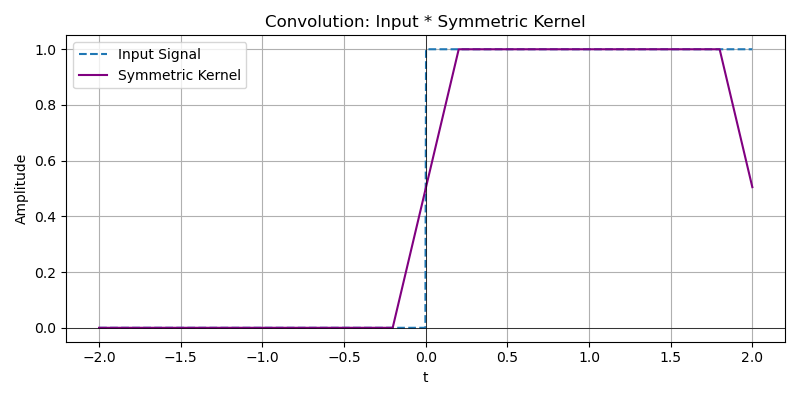
\includegraphics[width=\textwidth]{figs/2.png}
        \caption{Convolution with Symmetric Kernel}
    \end{subfigure}
    \vskip\baselineskip
    \begin{subfigure}{0.45\textwidth}
        \centering
        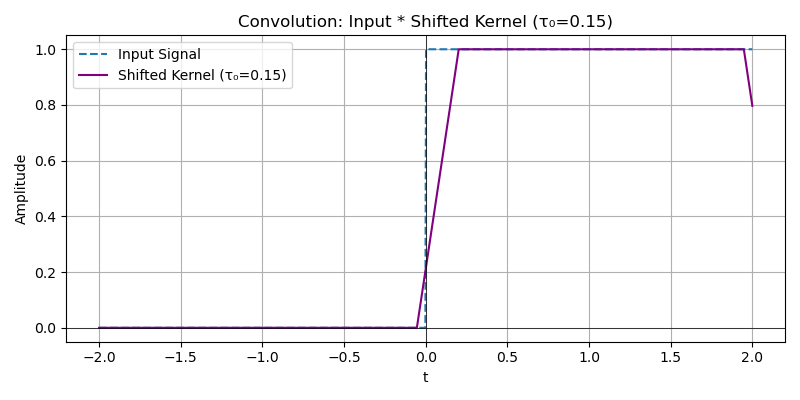
\includegraphics[width=\textwidth]{figs/3.png}
        \caption{Convolution with Shifted Kernel $(\tau = 0.15)$}
    \end{subfigure}
    \caption{Convolution of the Step Function with Different Kernels}
\end{figure}

\subsection{Delta Function Convolution}
Next, we show the convolution of the delta function (approximated by a narrow spike) with the same set of kernels.

\begin{figure}[h!]
    \centering
    \begin{subfigure}{0.45\textwidth}
        \centering
        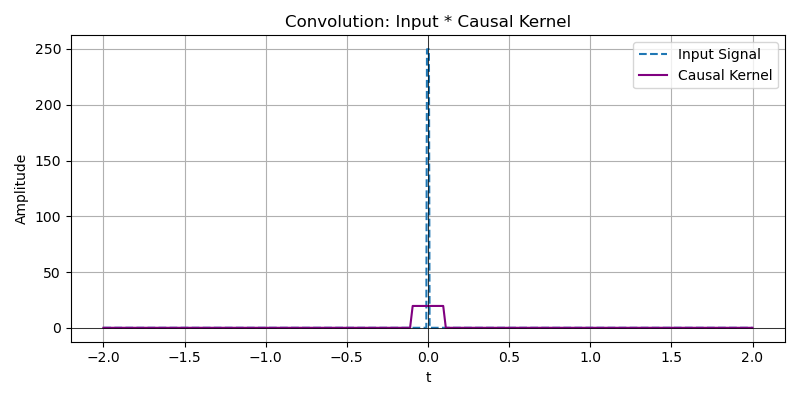
\includegraphics[width=\textwidth]{figs/4.png}
        \caption{Convolution with Causal Kernel}
    \end{subfigure}
    \hfill
    \begin{subfigure}{0.45\textwidth}
        \centering
        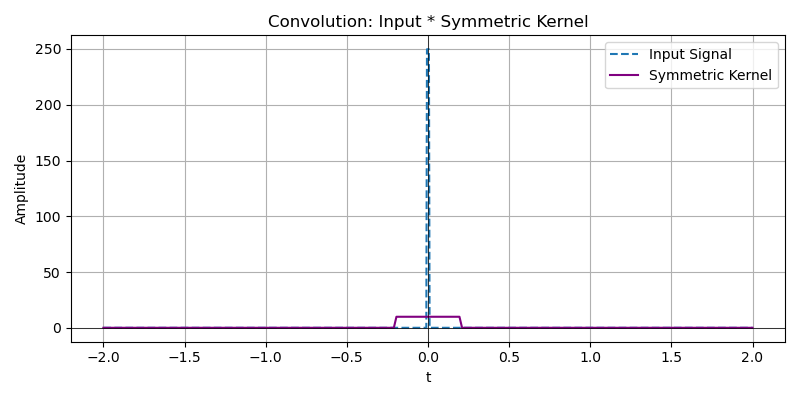
\includegraphics[width=\textwidth]{figs/5.png}
        \caption{Convolution with Symmetric Kernel}
    \end{subfigure}
    \vskip\baselineskip
    \begin{subfigure}{0.45\textwidth}
        \centering
        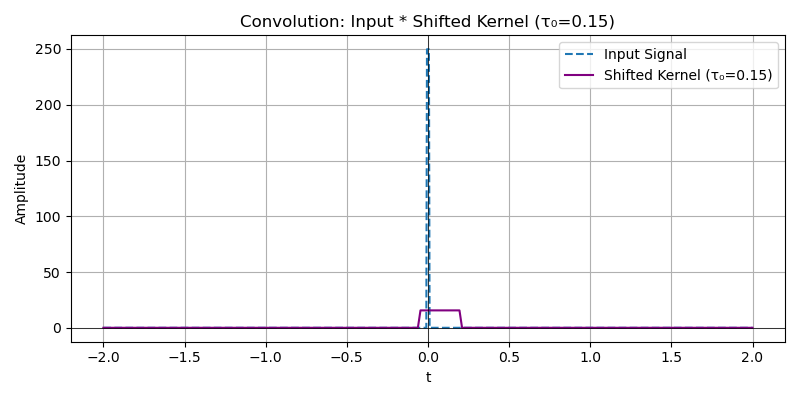
\includegraphics[width=\textwidth]{figs/6.png}
        \caption{Convolution with Shifted Kernel $(\tau = 0.15)$}
    \end{subfigure}
    \caption{Convolution of the Delta Function with Different Kernels}
\end{figure}

\section{Conclusion}
The above convolution results demonstrate how the step and delta functions interact with different kernel types, providing insights into signal processing and filtering effects. The causal kernel introduces a delay, the symmetric kernel smooths the signal, and the shifted kernel introduces a time shift.

\end{document}

